\documentclass[a4paper,12pt]{article}

% Packages
\usepackage[english]{babel}           
\usepackage[latin1]{inputenc}       	% speciale karakters
\usepackage{graphicx} 				% figuren
\usepackage[hyphens]{url}
\usepackage{hyperref}
\usepackage{subfigure}
\usepackage{amssymb}
\usepackage{amsmath}
\usepackage{graphicx}
\usepackage[font=small,format=plain,labelfont=bf,up,textfont=it,up]{caption}
\usepackage{float}
\usepackage[bottom]{footmisc}
\usepackage[T1]{fontenc}
\usepackage{lastpage}
\usepackage{fancyhdr}
\usepackage{listings}
\usepackage{hvfloat}
\usepackage{color}

\definecolor{mygreen}{rgb}{0,0.6,0}
\definecolor{mygray}{rgb}{0.5,0.5,0.5}
\definecolor{mymauve}{rgb}{0.58,0,0.82}

\lstset{ %
	backgroundcolor=\color{white},   % choose the background color; you must add \usepackage{color} or \usepackage{xcolor}
	basicstyle=\footnotesize,        % the size of the fonts that are used for the code
	breakatwhitespace=false,         % sets if automatic breaks should only happen at whitespace
	breaklines=true,                 % sets automatic line breaking
	captionpos=b,                    % sets the caption-position to bottom
	commentstyle=\color{mygreen},    % comment style
	deletekeywords={},            % if you want to delete keywords from the given language
	escapeinside={\%*}{*)},          % if you want to add LaTeX within your code
	extendedchars=true,              % lets you use non-ASCII characters; for 8-bits encodings only, does not work with UTF-8
	frame=single,                    % adds a frame around the code
	keepspaces=true,                 % keeps spaces in text, useful for keeping indentation of code (possibly needs columns=flexible)
	keywordstyle=\color{blue},       % keyword style
	language=Octave,                 % the language of the code
	morekeywords={*,...},            % if you want to add more keywords to the set
	numbers=left,                    % where to put the line-numbers; possible values are (none, left, right)
	numbersep=5pt,                   % how far the line-numbers are from the code
	numberstyle=\tiny\color{mygray}, % the style that is used for the line-numbers
	rulecolor=\color{black},         % if not set, the frame-color may be changed on line-breaks within not-black text (e.g. comments (green here))
	showspaces=false,                % show spaces everywhere adding particular underscores; it overrides 'showstringspaces'
	showstringspaces=false,          % underline spaces within strings only
	showtabs=false,                  % show tabs within strings adding particular underscores
	stepnumber=1,                    % the step between two line-numbers. If it's 1, each line will be numbered
	stringstyle=\color{mymauve},     % string literal style
	tabsize=2,                       % sets default tabsize to 2 spaces
	title=\lstname                   % show the filename of files included with \lstinputlisting; also try caption instead of title
}

% Optional settings
\setlength{\hoffset}{-1.2cm}   
\addtolength{\textwidth}{2.5cm}
\setlength{\voffset}{-1.2cm}
\addtolength{\textheight}{2.5cm}

\setcounter{tocdepth}{3}
\setcounter{secnumdepth}{3}
\def\thesection{\arabic{section}}

\pagestyle{fancy}
\lhead{Group 40}
\rhead{Report: Error Correction in Digital Video}


\begin{document}
\begin{titlepage}

\fontsize{12pt}{14pt}
\selectfont

\begin{center}


\includegraphics[height=3cm]{includes/images/UGent}

\vspace{0.5cm}

Faculty of Engineering\\
Master of Science in Computer Science\\

\vspace{4.0cm}

\fontseries{bx}
\fontsize{17.28pt}{21pt}
\selectfont

\textbf{DESIGN OF MULTIMEDIA APPLICATIONS} \\
\vspace{40pt}

\hrule
\vspace{20pt}
\textsc{Group 40}\\
\vspace{10pt}
\textbf{Report: Error Correction in Digital Video}\\
\vspace{20pt}
\hrule

\vspace{25pt}

\fontseries{m}
\fontsize{12pt}{14pt}
\selectfont

\vspace{5.0cm}

\fontseries{m}
\fontsize{12pt}{14pt}
\selectfont

\hspace{0.5cm} Group 40
\textbf{ 
	\hfill\textsc{Naessens} Tom\\
	\hfill\textsc{Van Den Bossche} Pieter\\
	\hfill\textsc{Wijnant} Joris\\
}
\end{center}
\end{titlepage}

\section{Explanation and clarification of algorithms}
\subsection{2.B}
The implementation for 2.B is almost exactly the same as 2.A, as described in the assignment. The difference lies within the referenceblocks. Where in 2.A it was expexted that every missing macroblock had no missing neighbouring blocks, in 2.B these neighbouring blocks could be missing. In the implementation for 2.N, when neighbouring blocks are missing, the algorithm looks further ahead in every direction untill it finds a not-missing macroblock. This is stored in a datastructure that keeps a pointer to the block itself and the distance it was found at. We call structures `spatial\_reference\_block'. The four relevant blocks (top, right, bottom, left) get provided to our processing algorithm in another datastructure called the `spatial\_reference\_blocks'. Our algorithm itself will then make a weighted mean calculation of the, in best case, four values provided from the edges of the blocks in the `spatial\_reference\_blocks'. This will be done for every pixel in the missing block. In what follows we will provide the pseudocode for 2.B.

The following pseudocode describes our method:
\begin{lstlisting}
main:
	blocks = get_4_surrounding_ref_macroblocks(missing_block_id);
	
	for pixel in missing_block:
		pixel_chroma  = calculate_chrome_value(blocks);
		pixel_luma    = calculate_chrome_value(blocks);
		
get_4_surrounding_ref_macroblocks(missing_block_id):
	while left->isMissing:
		left++
	blocks.add(left)
	
	#... etc for top, right and bottom
	
	return blocks
\end{lstlisting}

A possible optimalisation, which we didn't implement, would be to search not only horizontally and vertically, but also diagonally. This allows us to extract more information from the surrounding macroblocks and would let us extract a better result.

\subsection{2.C}
\paragraph*{Disclaimer}
We did our best to implement this function, but we did not succeed. If we decoded our movie sequence with the simple error pattern, some areas became pink while the others remained green. When running with a complex error pattern, we got segfaults. So there is certainly something wrong with our code. For the rest of this report, we will try to predict the behavior of this method. 

\paragraph{Concept of implementation}
We have looked at many papers to get some idea on how to implement this method. The most promissing technique seemed to be the usage of the sobel operator which is described, or an alternative operator like the Prewitt operator, in almost every paper concerning edge detection. The way we used the sobel operator was by convolving the operator with every 3x3-block along the edges of the excisting neighbouring macroblocks. From this result every 3x3 convolution gave us an x and y value which could be used to calculate the general angle of the edge in the 3x3 block. We used a weighted consensus to determine which "general angle" was most likely to go through the missing block and also took into account the possibility of there being no angle at all. In what follows we will provide the pseudocode for 2.B.

\begin{lstlisting}
main:
	blocks = get_8_surrounding_ref_macroblocks(missing_block_id);
	angle = get_angle(blocks)
	extrapolate_missing_block(missing_block_id, angle)
	
	get_8_surrounding_ref_macroblocks(missing_block_id):
	if(missing_block->left.is_not_missing())
	blocks.add(left)
	#... etc for other 7 blocks
	
	return blocks

get_angle(blocks):
	consensus_array[8]

	for(block in blocks)
		for(every 3x3 block along relevant edge of block ALIAS 3B)
			Xs = convolve(sobelX, 3B)
			Ys = convolve(sobelY, 3B)
			magnitude = |Xs, Ys|
			angle = arctan(Xs, Ys)
			consensus_array[integer_division(angle, 22.5)] += magnitude
		
	return angle with highest consensus_array[i] value

extrapolate_missing_block(missing_block_id, blocks, angle):
	for(pixel in missing block, from left top to right bottom)
		pixel->luma = calculated_weighted_luma_value(angle, blocks)
		pixel->chroma = calculated_weighted_luma_value(angle, blocks)
\end{lstlisting}

When the general angle was determined, which we choose it to be a multiple of 22.5�, we then try to extrapolate the surrounding blocks through the missing block. We are pretty sure the angle calculation is done correctly and the angles it provides are correct. The extrapolation method is quite complex and tricky because the ``conditional'' case keep piling onto one another and it was easy enough to slip up somewhere. We did a search for the mistake we made, but sadly did not find it.

\subsection{3.C}
3.C is a combination of the previous methods 3.A and 3.B. As a base, we started with the code from 3.B. As we couldn't assume the neighbouring macroblocks weren't missing, we expanded the code: instead of using the motion vectors from the top, left, right and bottom block, we went looking for existing macroblocks spiralwise around the missing macroblock. We added each macroblock we found to a list. From the moment we found 10 macroblocks, we stopped our search. We then added 2 extra macroblocks: One with a motion vector which is the average of all the motion vectors of the non-missing macroblocks and another with the motion vector $\left(0, 0\right)$. This last macroblock matches the algorithm described in 2.A.

For every macroblock in the list, we generated the ``shifted'' macroblock and calculated, using the boundary matching, an error score. We then replaced the missing macroblock with its shifted corresponding macroblock with the smallest error.

The following pseudocode describes our method:
\begin{lstlisting}
list = get_spiralwise_10_surrounding_macroblocks();
block = get_block_with_average_motion_vector();
add_block_to_list();
block = get_block_with_zero_motion_vector();
add_block_to_list();

error = Int.MAX;
for block in list:
	new_error = calculate_boundary_matching_error();
	if new_error < error:
		error = new_error;
		copy_current_block_to_missing_block();
\end{lstlisting}

The reason why we chose for this method is because we wanted to fit as many different macroblocks as possible into the comparison. This method unifies all the algoritms used in 3.A, 3.B and adds a method of its own. The more macroblocks, the more information we can use for our error correction and, hopefully, the better the error correction will be.

\section{Measurement results}
\subsection{Time results}
To be able to compare time needed to decode and correct of the given video sequences, we had to normalize the total time: We took the total decoding and error correcting time and divided this by the number of frames in the video sequence to obtain the average decoding and error-correcting time per frame. We then took this time and divided it by the amount of macroblocks in the frame and, lastely, multiplied this small number with $1000$. This way, we become the average time to decode one frame of the given video sequence, as if the frame would be $1000$ macroblocks large. With this method, we can compare the given video sequences without being influenced by the length or dimensions of the given video. Our timing resulsts can be seen in figure \ref{timing} at page \pageref{timing}.

\begin{figure}[ht!]
	\centering
	\includegraphics[width=\textwidth]{includes/images/tijd}
	\caption{Decoding time in ms for the given video sequences per frame, normalized to 1000 macrobloks per frame. This plot has also been added to the attachements in a larger size.}
	\label{timing}
\end{figure}

The first noticable difference in the plot are the differences between the different video sequences. The natural sequence takes in (in all but one measurement) the longest to decode and error correct. This sequence is closely followed by our group sequence. Looking at our algorithms, the amount of motion in a frame should not cause longer error correction. However, the motion estimation decoding process may result in a slightly longer time for video sequences with more movement. As we didn't succeed in finishing 2.C, we don't have any timing measurements from this method. However, we think that these timings take a lot longer than any of the other methods because of it's high complexity.

The second difference is that 3.C takes the longest time. This makes sense, because (apart from 2.C) 3.C is the most complex method. Because we circle spiralwise around the missing block, it can take a while before ``neighbouring'' blocks are found. 

If we compare the simple with the complex error patters, we notice a slightly longer error correcting time accross all sequences. This too is logical, because there are simply more macroblocks to correct. If we look into the differences more into detail; we notice expected results. For example, decoding a complex frame with 2.B takes a little longer then a simple frame. This because we have to search ``further'' in the 4 directions when there aren't any neighbours available. The same can be said for 3.C: We have to search (spiralwise) further as the close neigbours can be unavailable.

Comparing the 2.x methods with the 3.x, we do not (apart from 3.C as explained before) notice a notificant amount of difference.

\subsection{Quality results}
The results from our quality measurements can be found in figure \ref{psnr} on page \pageref{psnr}.
What immediately comes to attention is that the synthetic video has the highest PSNR of all video sequences for every method. If we look look at this video, we notice that it is a rather static movie without too many moving frames or scenes with much detail. These qualities make sure the error correcting part is not as hard as for the other videos. Our group video has slightly more moving frames, so the error correction is in general a bit worse. The worst video is the natural clip as the scenes rapidly follow eachtother and contain a lot of motion and detail.

\begin{figure}[ht!]
	\centering
	\includegraphics[width=\textwidth]{includes/images/psnr}
	\caption{PSNR for the given video sequences. This plot has also been added to the attachements in a larger size.}
	\label{psnr}
\end{figure}

Obviously, the complex methods are worse than the simple methods as we do not have as much information available.

The values for 2.C are not representative for the result that we should have become. When looking at the decoded video sequence, we noticed a lot of pink and bright green squares, caused by a bug in our code. We however expect that 2.C would have been the best method in the 2.x series as 2.C uses a much smarter data extraction method.

Comparing the 2.x with the 3.x, we notice that the PSNR values are a little bit higher for the 2.x series for the simple error patterns. The values for the complex error patterns are slightly better. This can be explained by the methods used: the 3.x methods look at previous frames to gather this information, while the 2.x methods look around the missing macroblocks. If a lot of macroblocks are missing, 3.x can still get information from ``close blocks'' in the past as these have been reconstructed at that moment, while 2.x methods have to grab data from ``further'' macroblocks. 

\section{Conclusion}
\subsection{Clear winner}
Purely judging by the PSNR and timing resulsts we have obtained, we wouldn't say that there is a clear winner. There are no outliers, neither in the PSNR plot nor in the timing plot. 
However, we do suspect that 2.C would obtain the best result, but would come with a time cost as this method is so complex. But as said before, we can't prove this.

\subsection{Visual inspection}
Visual inspection yields a different result. If we visually compare the 2.x with the 3.x series, we notice some big differences, in comparison to the difference in the PSNR rating. The error corrected frames from the 2.x methods were more ``blurry'' while the error corrected frames from the 3.x methods contained more detail. This is demonstrated in figure \ref{2bvs3c} on page \pageref{2bvs3c}. As you can see in the PSNR plot, there is not much difference between these two methods. However, it is a lot easier to recognize the woman's face in 3.C then in 2.B. We noticed the same behaviour in the other video sequences.

We can conclude that the PSNR is not always a good measure for a better quality video. The human brain also performs some sort of autocorrection, so we should not only look at the difference between the pixels, but also to what we can extract from the error corrected messages. 

\section{Client-side buffering}
Client-side buffering has both advantages and disadvantages. If we want a video to play realtime, we do not have the time to buffer video: the video should be displayed as soon as possible. This means that we have very little time for error correction. If an error is found, we should use simple and light error correction methods which are fast.

However, if we have a little time to let the video buffer, we have more time to make use of more complex error correcting algorithms, which are allowed to run relatively longer. The trick here is to make sure that the error correcting algorithms still are fast enough to display the video without interuption. We can't allow the playback to be much slower than the error correction, as this would mean that the video has to stop at intervals so the error correction and decoding can catch up. This would lead to a stuttering playback. The higher quality of error correction we want to apply, the longer the video should buffer before playback.

We conclude here that client-side buffering is a tradeoff between the speed a video can be shown (realtime, or with some delay) and the quality of the error corrected sequence.

\section{Highest PSNR for Bourne Ultimatum}
We obtained the following values for methods 2.B, 2.C and 3.C for the complex error pattern for the Bourne Ultimatum scene:

\begin{tabular}{c|c}
 & PSNR \\ 
\hline 
2.B & 27.43 \\ 
\hline 
2.C & / \\ 
\hline 
3.C & 28.45
\end{tabular} 

\newpage
\section*{Attachments}

\begin{figure}[ht!]
  \centering
  \includegraphics[angle=90]{includes/images/tijd}
  \caption{Decoding time in ms for the given video sequences per frame, normalized to 1000 macrobloks}
\end{figure}
  
\begin{figure}[ht!]
  \centering
  \includegraphics[angle=90]{includes/images/psnr}
  \caption{PSNR rating for the given video sequences}
\end{figure}

\begin{figure}[htp]
	\centering
	\subfigure[2.B complex]{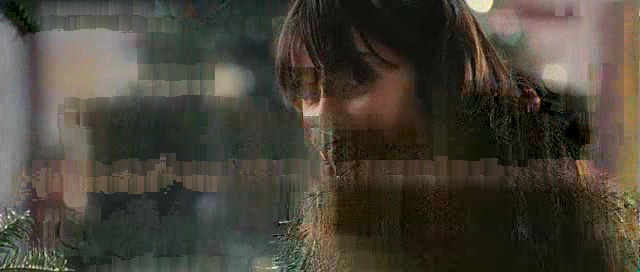
\includegraphics[width=30pc]{includes/images/visual_comp_1}}
	\subfigure[3.C complex]{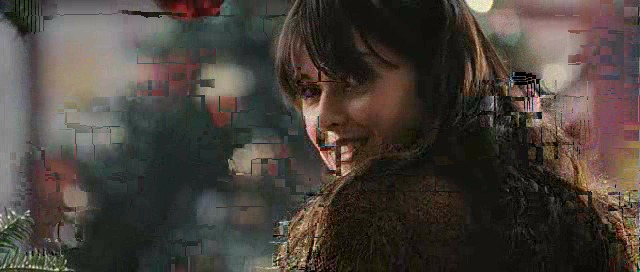
\includegraphics[width=30pc]{includes/images/visual_comp_2}}
	\caption{Comparison of method 2.B with 3.C for the complex error pattern}
	\label{2bvs3c}
\end{figure}


\end{document}
